\chapter{Pruebas de funcionalidad}\label{chapter:implementation}
En este capítulo se realizan un conjunto de pruebas para demostrar el buen funcionamiento de las herramientas implementadas y así evidenciar el cumplimiento de los
objetivos planteados en este trabajo.
Las pruebas se realizaron en dos dispositivos Android físicos y uno emulado desde Android Studio para abarcar la mayor cantidad de casos posibles\\
Los dispositivos tienen las siguientes prestaciones:\\
\section{Prestaciones de los dispositivos sobre los que se ejecutaron las pruebas}
\subsection{LG VELVET Android 13 [Dispositivo físico]}
\begin{itemize}
    \item 5.7 Gb RAM
    \item CPU Octa-Core a una frecuencia promedio por núcleo de 1.925 GHz
\end{itemize}
\subsection{Samsung Galaxy S23 Ultra Android 14 [Dispositivo físico]}
\begin{itemize}
    \item 8.0 Gb RAM
    \item CPU Octa-Core a una frecuencia promedio por núcleo de 2.57 GHz
\end{itemize}

\subsection{Google Pixel 4 Android 10 [emulador]}
\begin{itemize}
    \item 2.0 Gb RAM
    \item CPU Quad-Core
\end{itemize}


\section{Importación de un mapa}
\begin{figure}[h]
    % \centering
    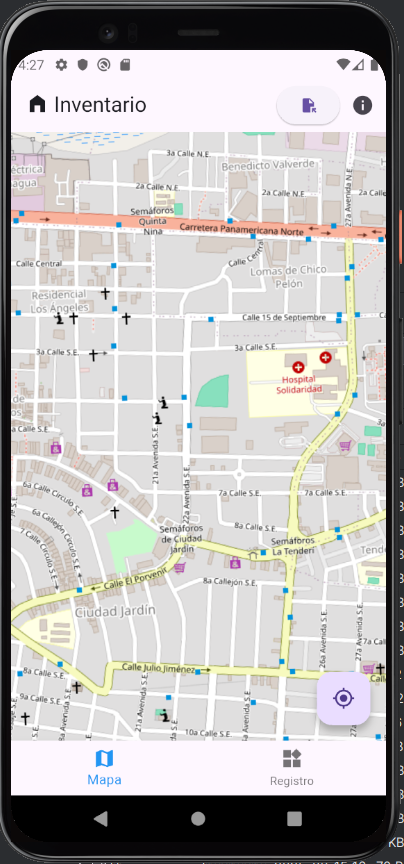
\includegraphics[width=0.3\textwidth]{Graphics/Capitulo 4/Pixel 4 [emulador]/4.2/1.png}
    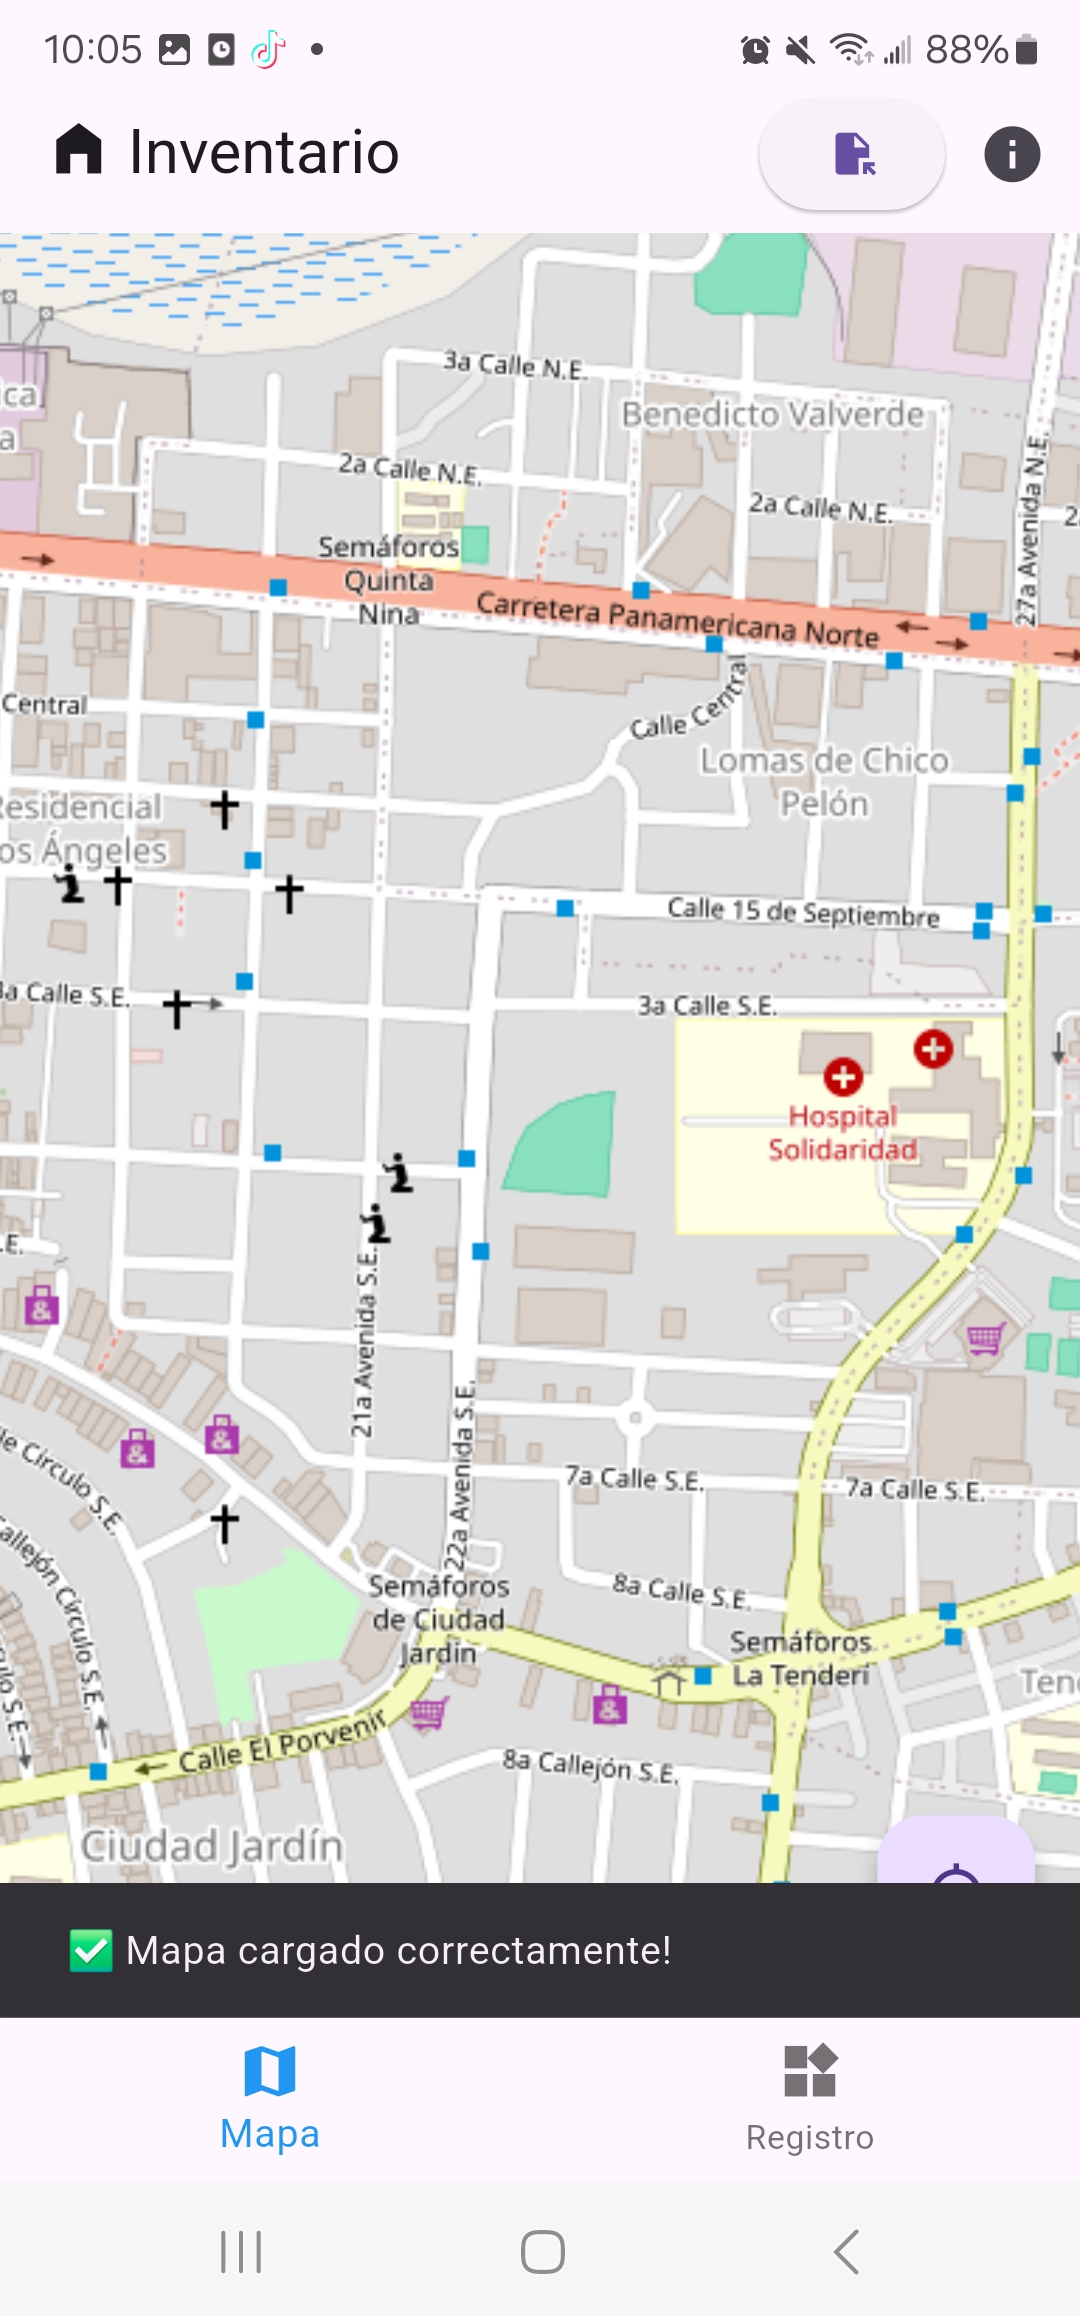
\includegraphics[width=0.3\textwidth]{Graphics/Capitulo 4/Galaxy S23 Ultra Android/4.2/3.jpg}
    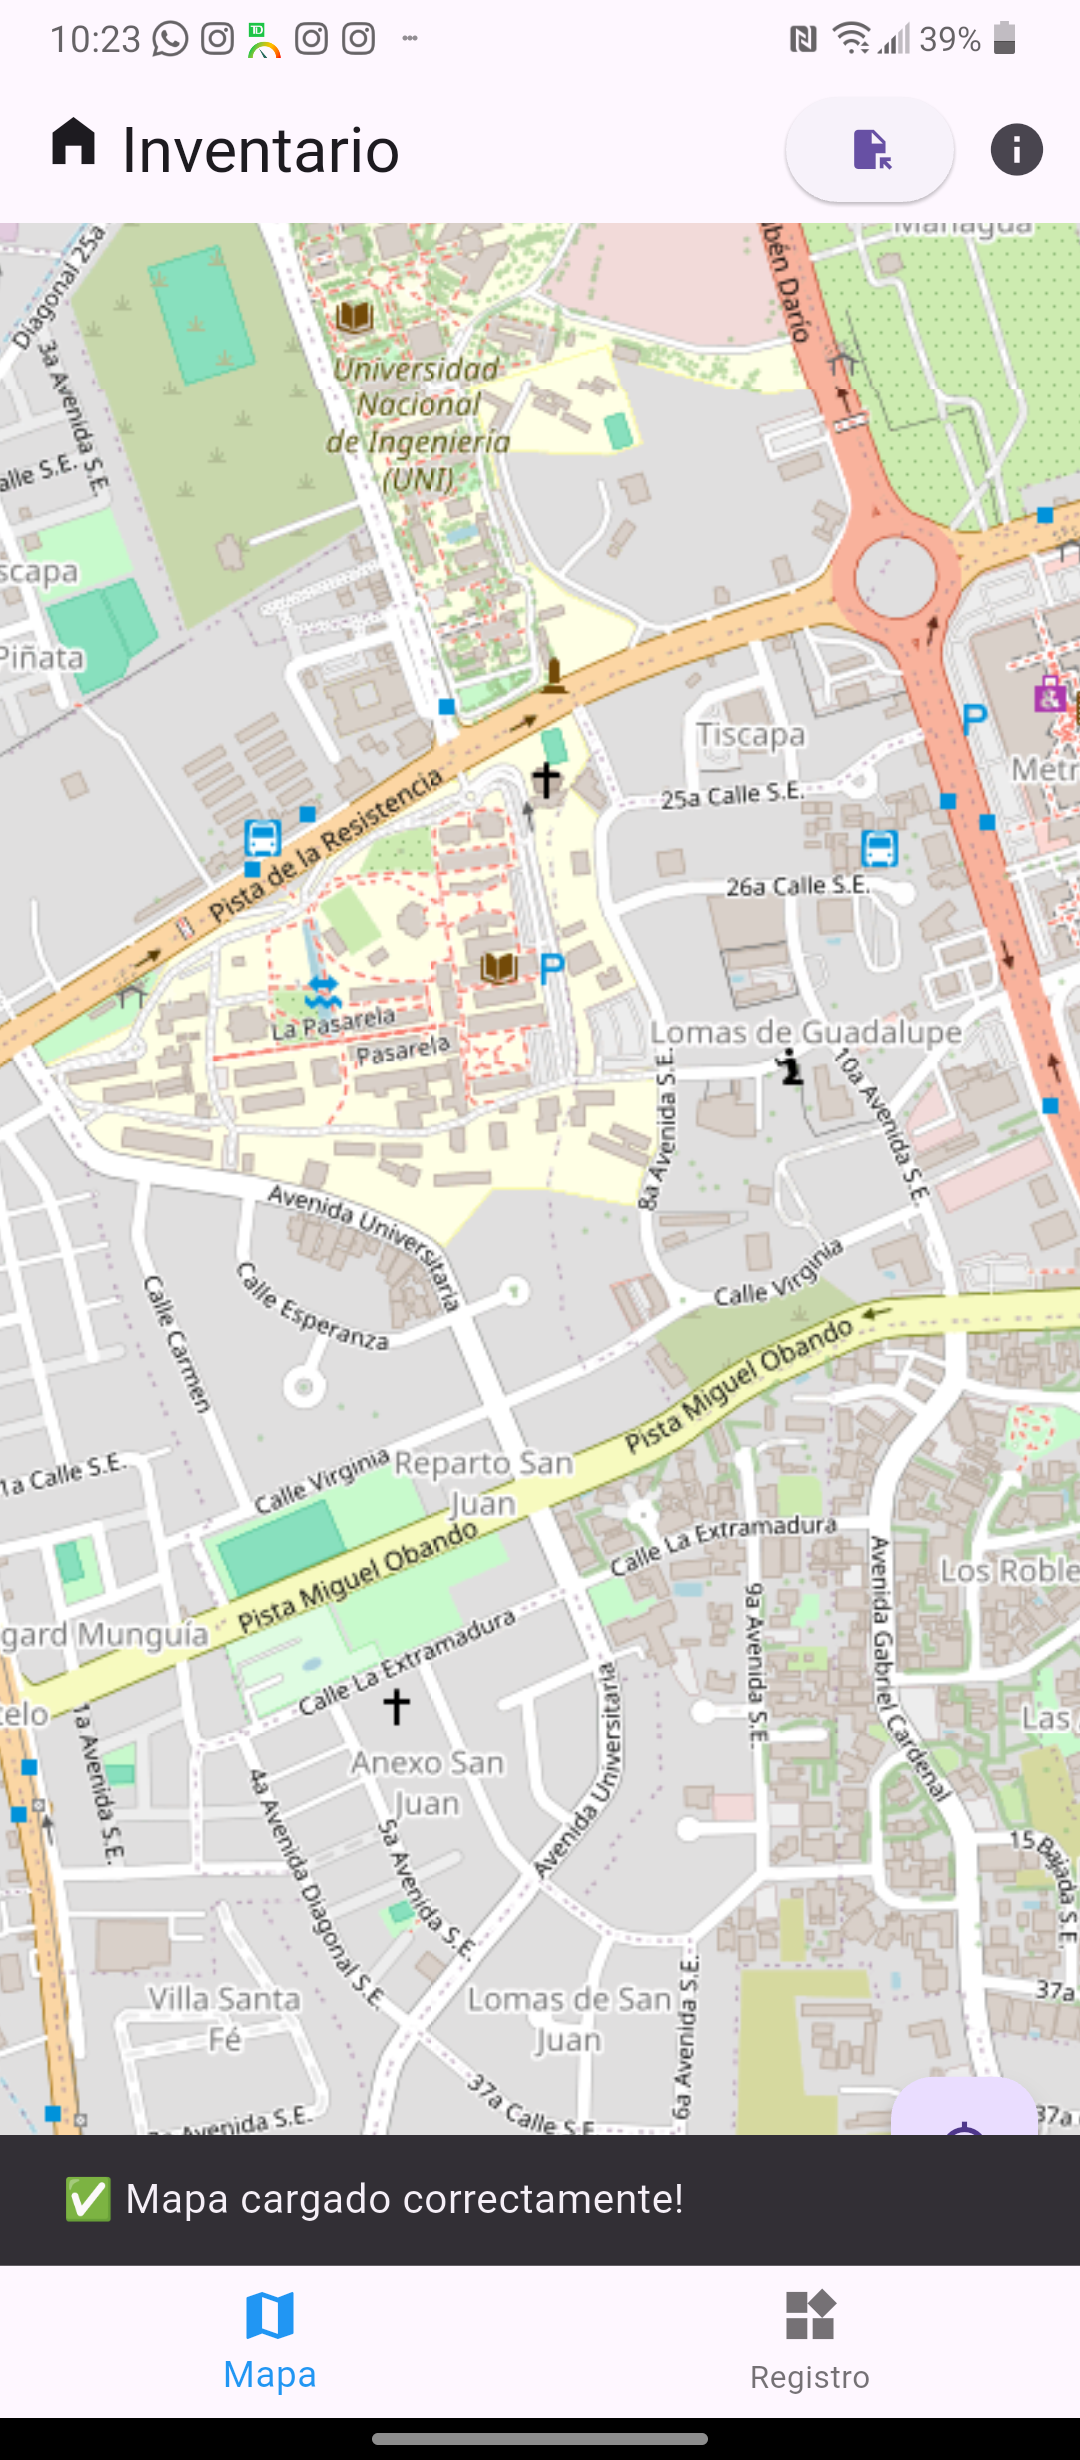
\includegraphics[width=0.3\textwidth]{Graphics/Capitulo 4/LG Android 13/4.2/2.png}
    \caption{Prueba de importacion de mapa}
    \label{fig:figura20}
\end{figure}
Esta constituye una prueba básica de las funcionalidades de la aplicación pero se debe tener en cuenta que también se está analizando compatibilidad
con versiones de Android antiguas como la 10 y esto es una prueba válida dada la inmensa cantidad de variaciones que se han hecho desde 2019(seis años atrás)
hasta la actualidad en actualizaciones del SO.

\pagebreak
\section{Importación de varias capas de delimitación, una de ellas con el formato de predios}
\begin{figure}[h]
    % \centering
    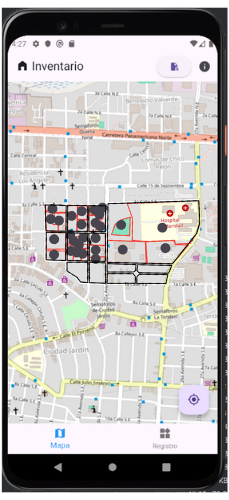
\includegraphics[width=0.3\textwidth]{Graphics/Capitulo 4/Pixel 4 [emulador]/4.3/1.png}
    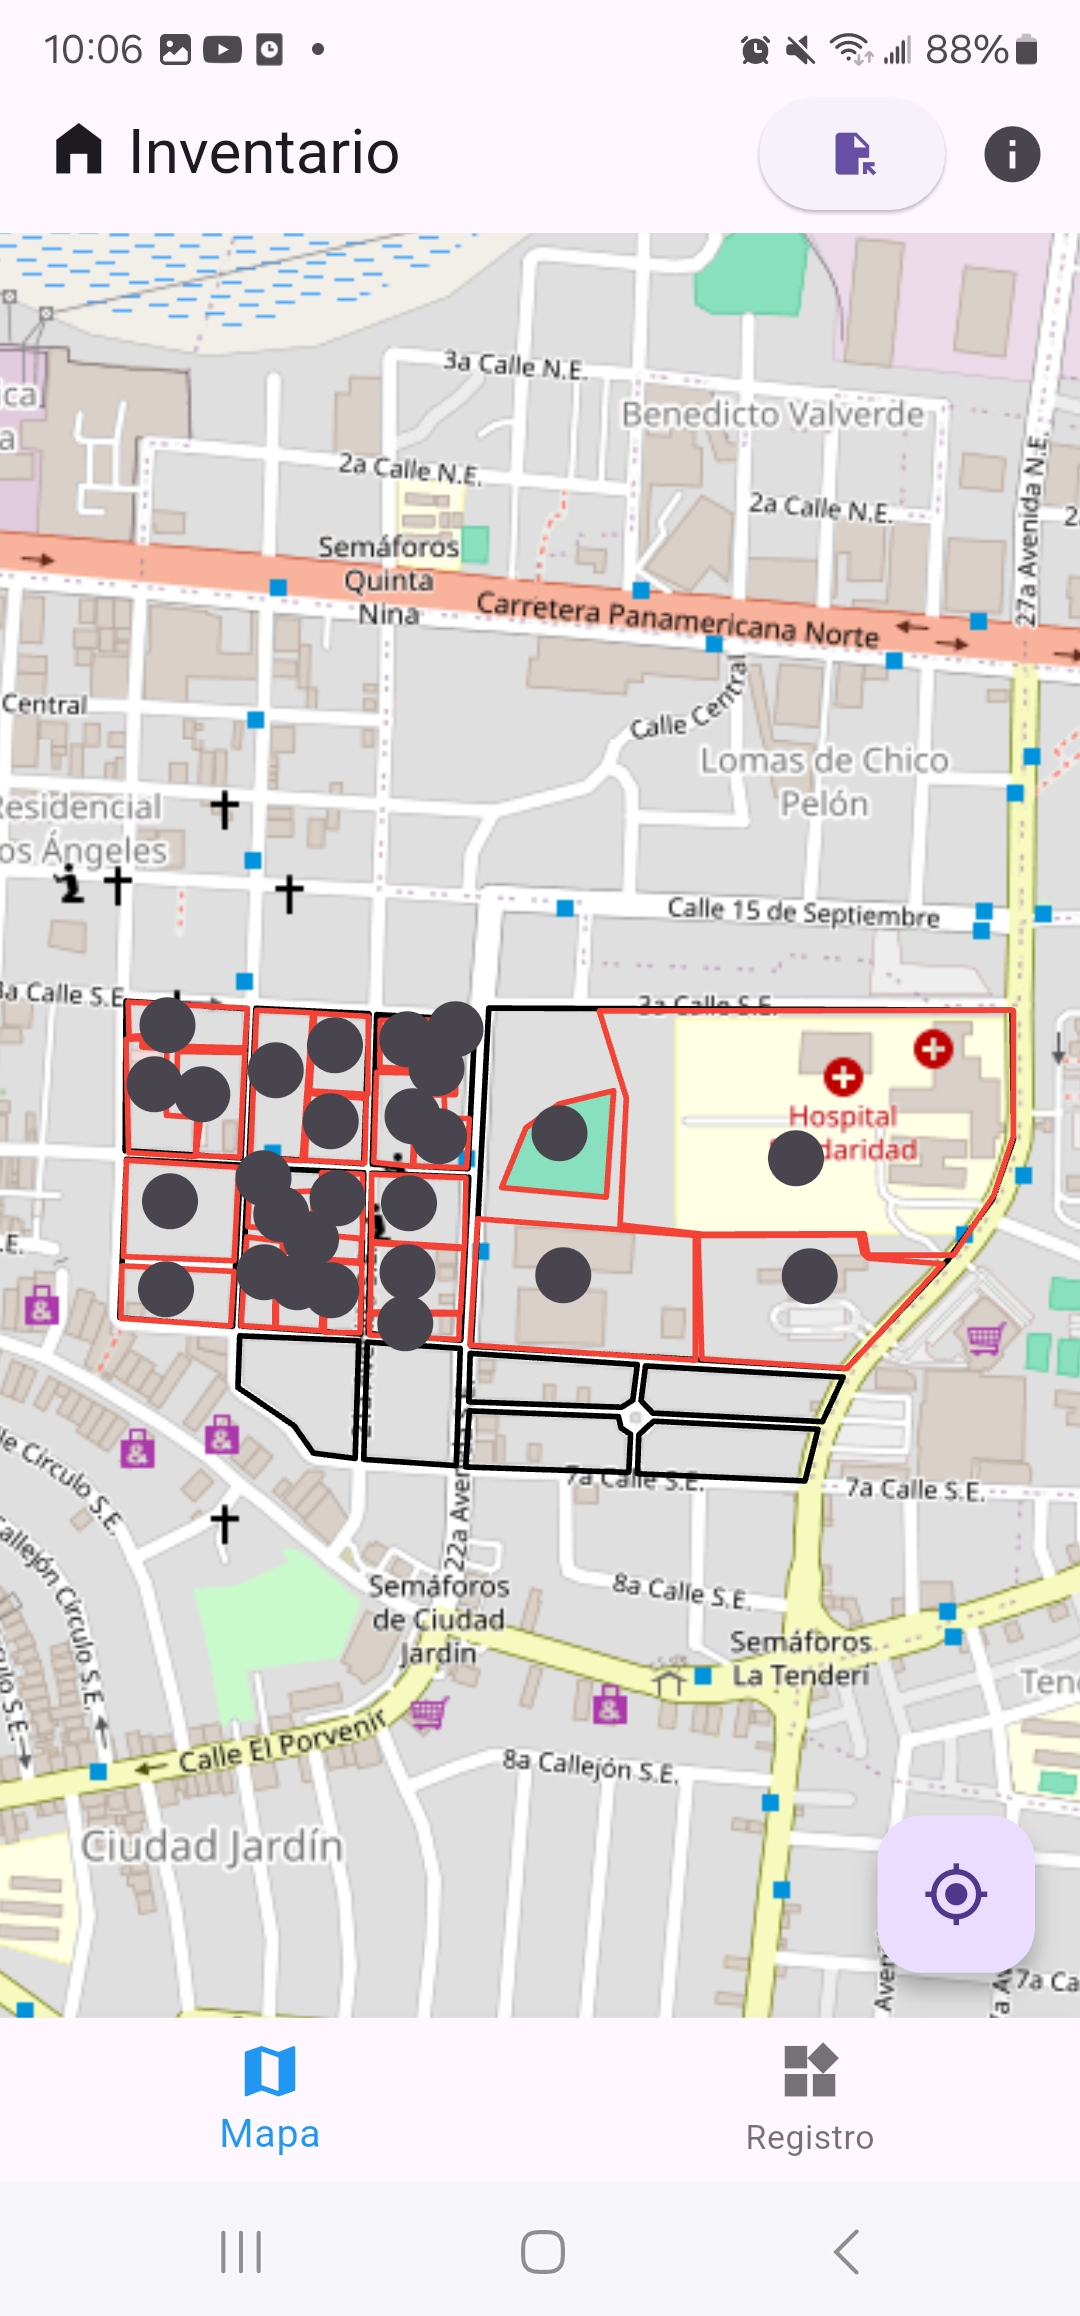
\includegraphics[width=0.3\textwidth]{Graphics/Capitulo 4/Galaxy S23 Ultra Android/4.3/4.jpg}
    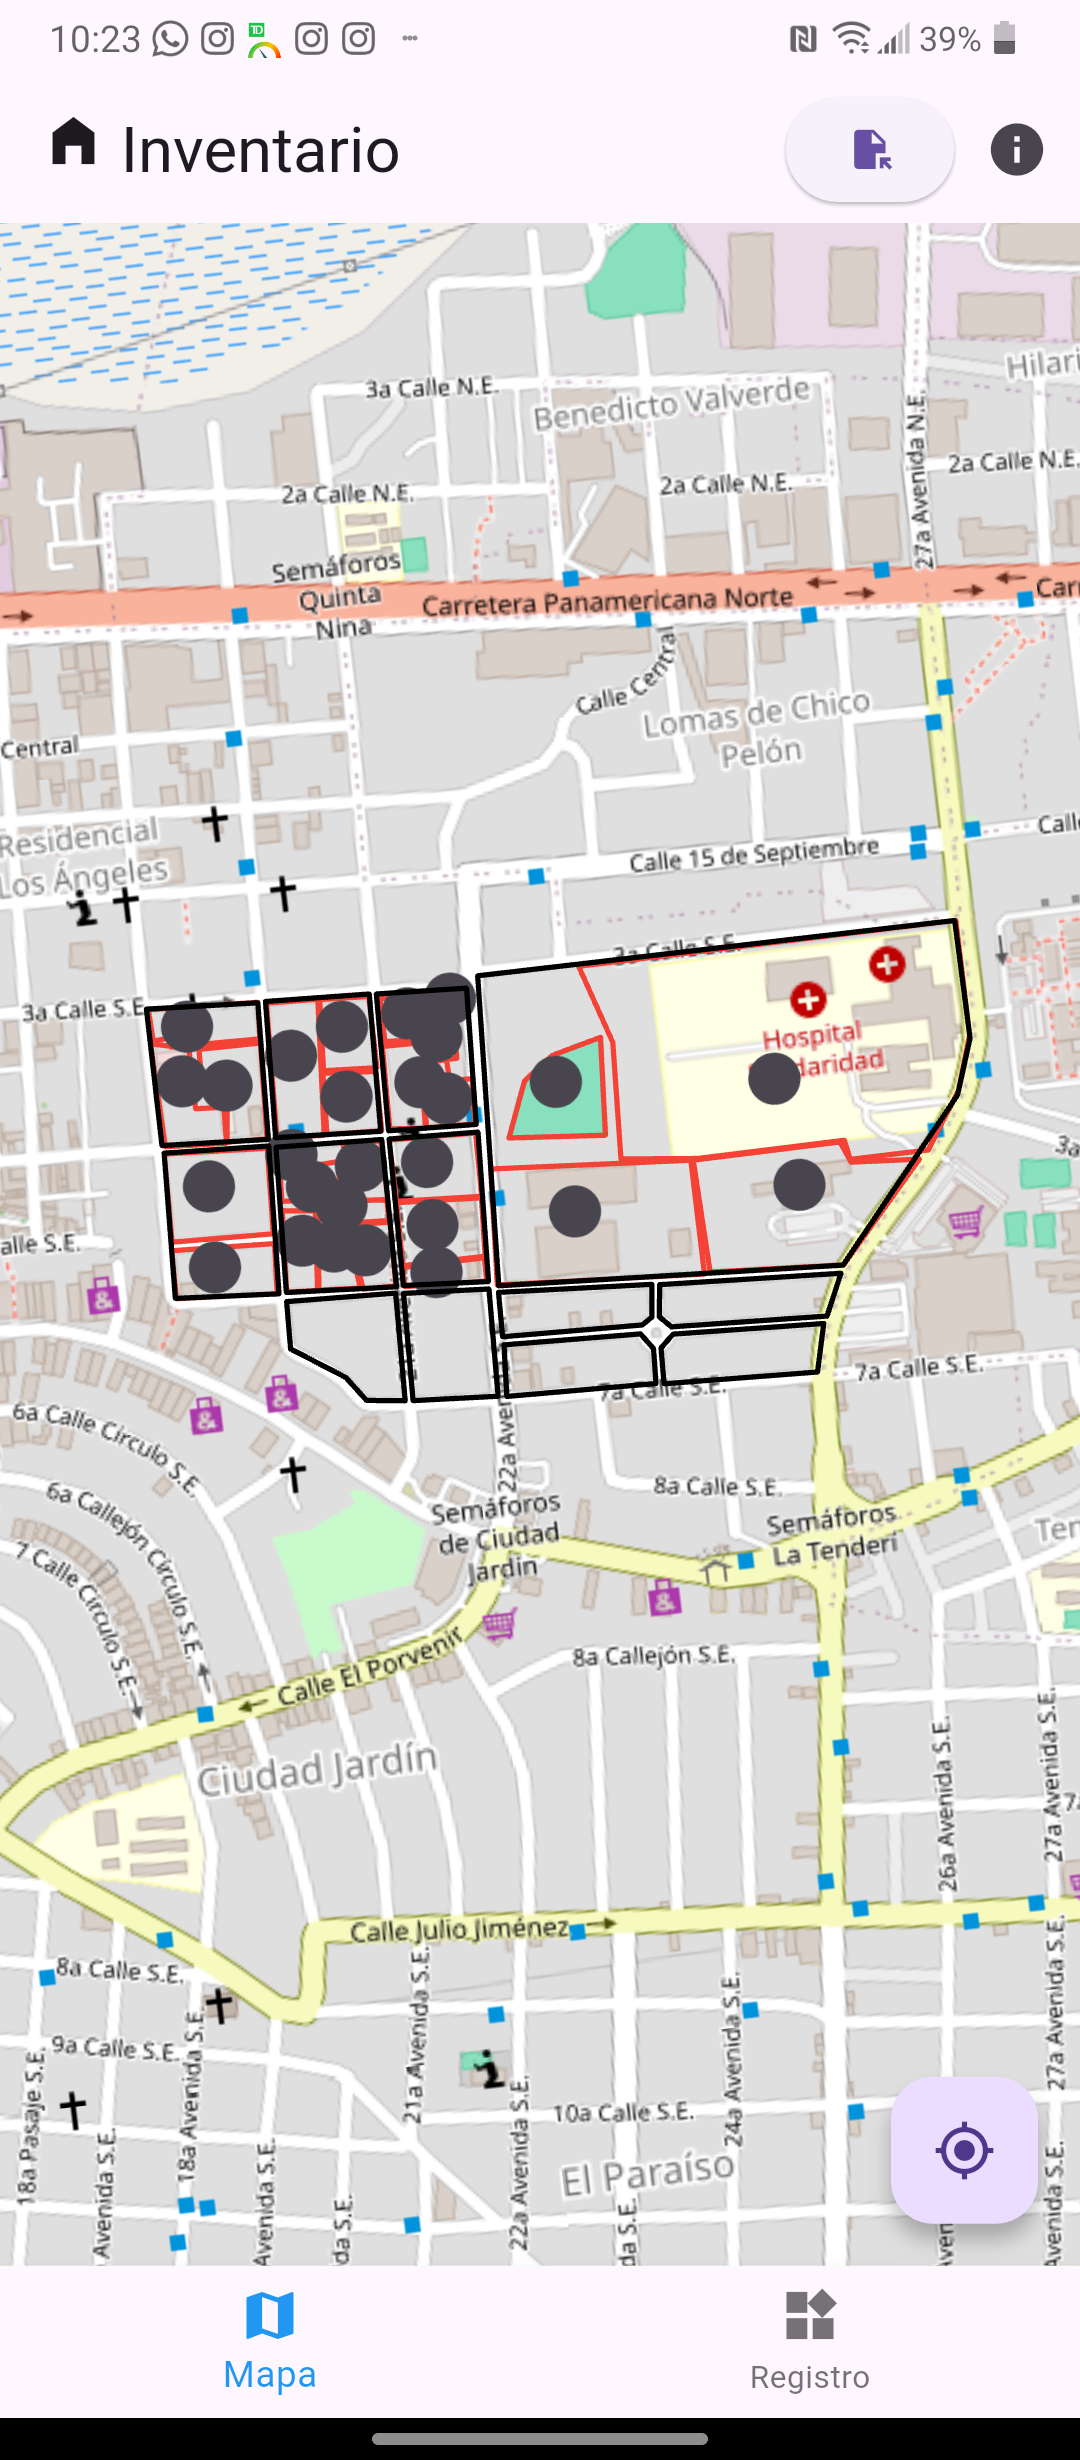
\includegraphics[width=0.3\textwidth]{Graphics/Capitulo 4/LG Android 13/4.3/1.png}
    \caption{Prueba de importacion de capa de delimitaciones}
    \label{fig:figura21}
\end{figure}
Se probó la funcionalidad de importación de mapa y ahora de delimitaciones y resultó sin problemas en las tres versiones diferentes de Android. Hay que decir que tanto esta funcionalidad
como la de importar mapa, son no imprescindibles, ya que al abrirse la aplicación por primera vez, esta crea el directorio CADIC en la raíz del almacenamiento
del dispositivo, y dentro tres subdirectorios donde se pueden copiar las delimitaciones o el mapa y estos cargarán igualmente bien.

\pagebreak
\section{Validación de Formularios}
\begin{figure}[h]
    % \centering
    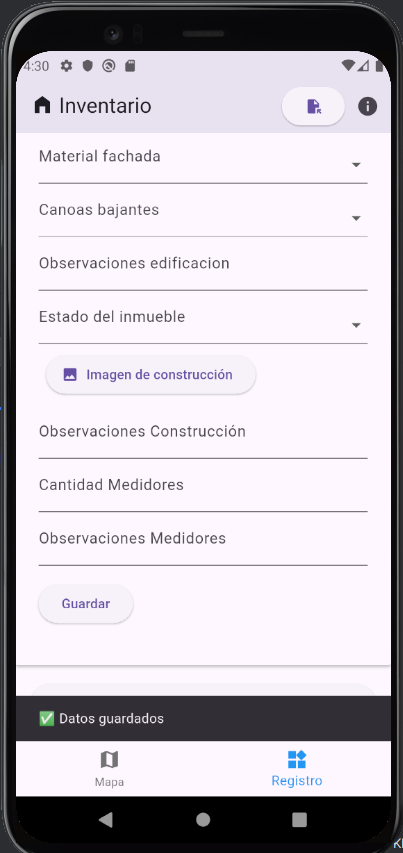
\includegraphics[width=0.3\textwidth]{Graphics/Capitulo 4/Pixel 4 [emulador]/4.4/1.png}
    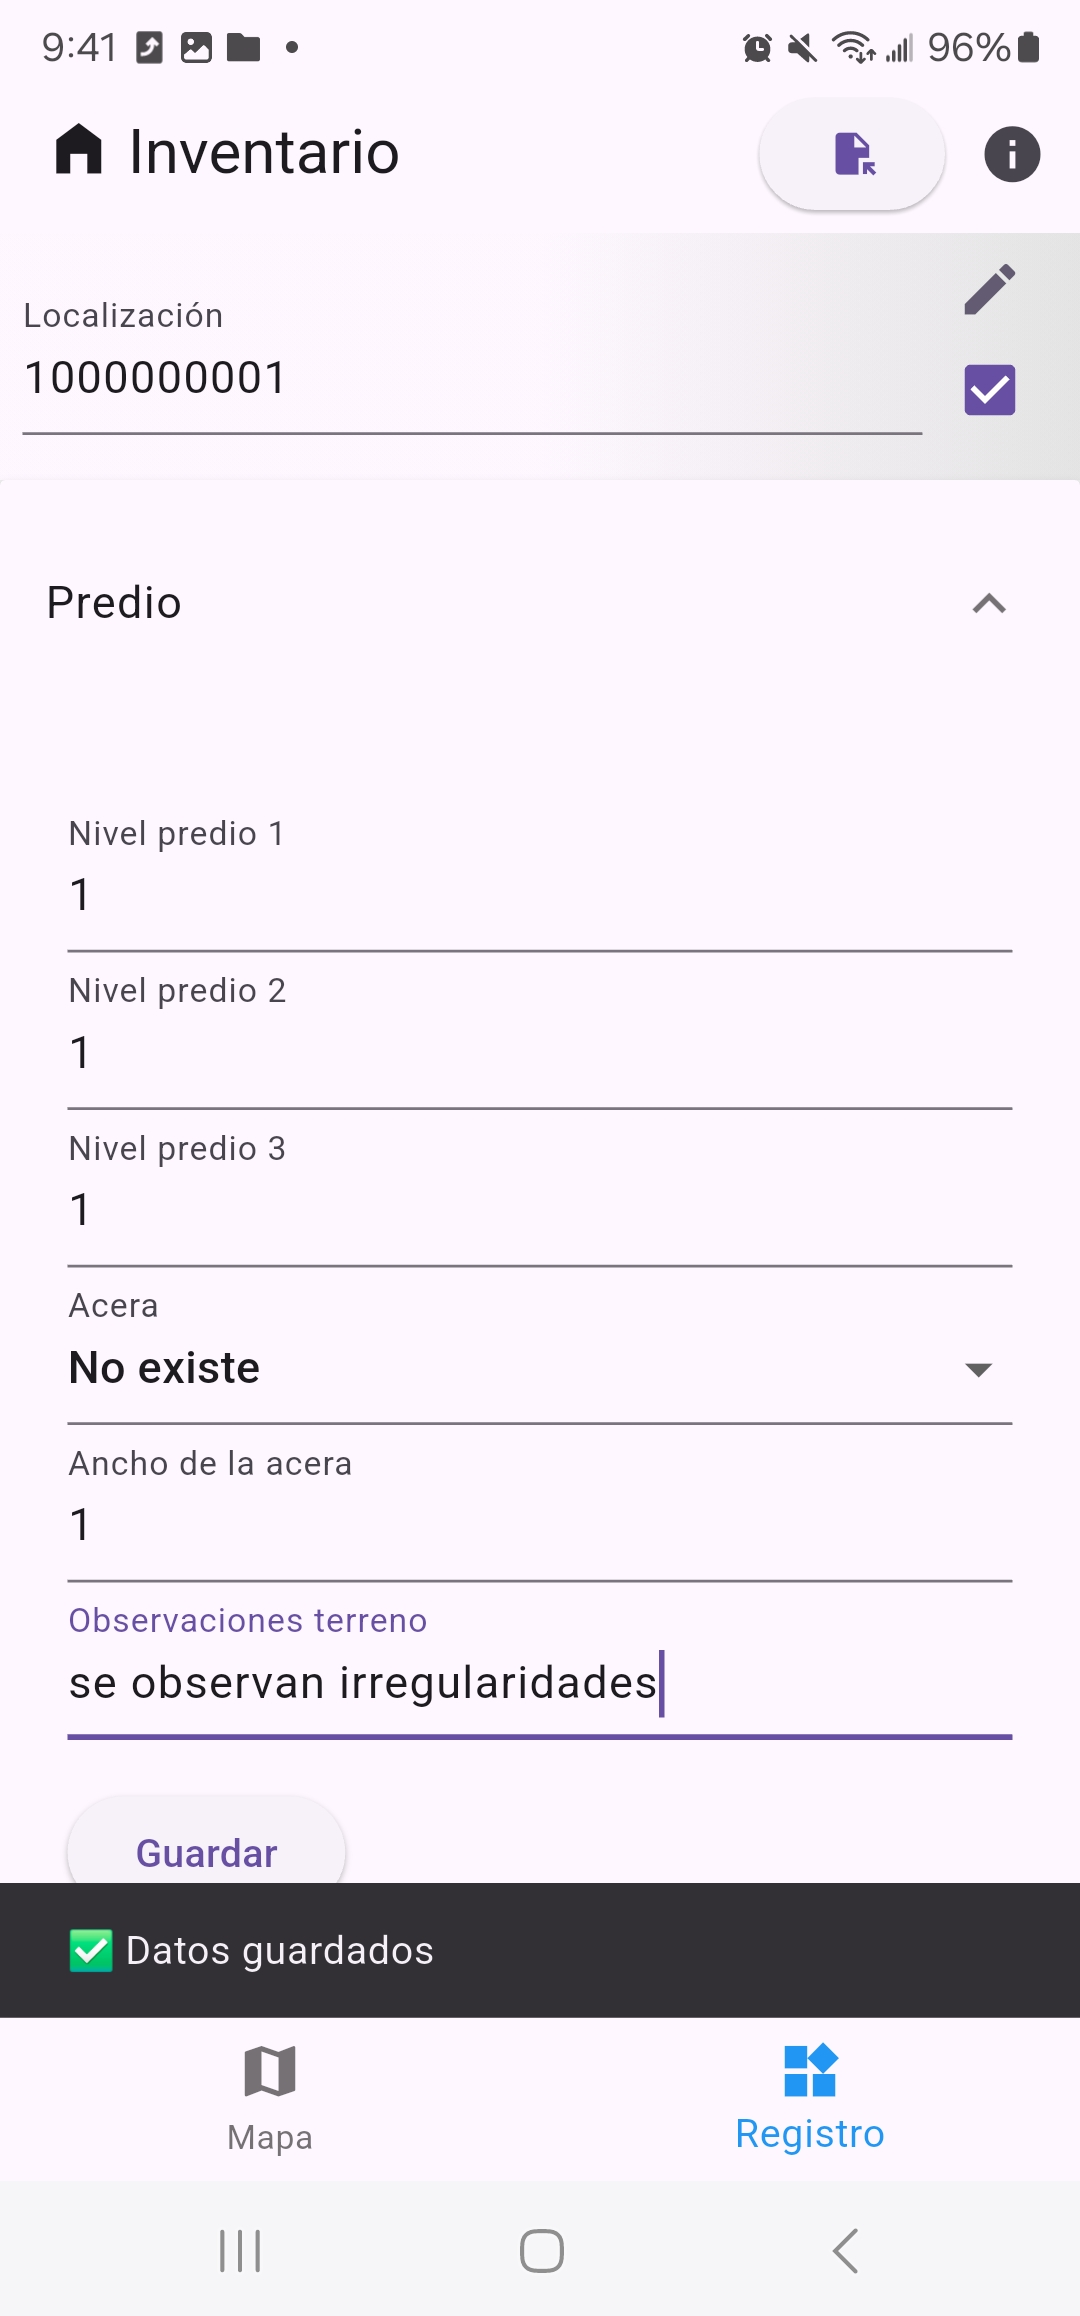
\includegraphics[width=0.3\textwidth]{Graphics/Capitulo 4/Galaxy S23 Ultra Android/4.4/1.jpg}
    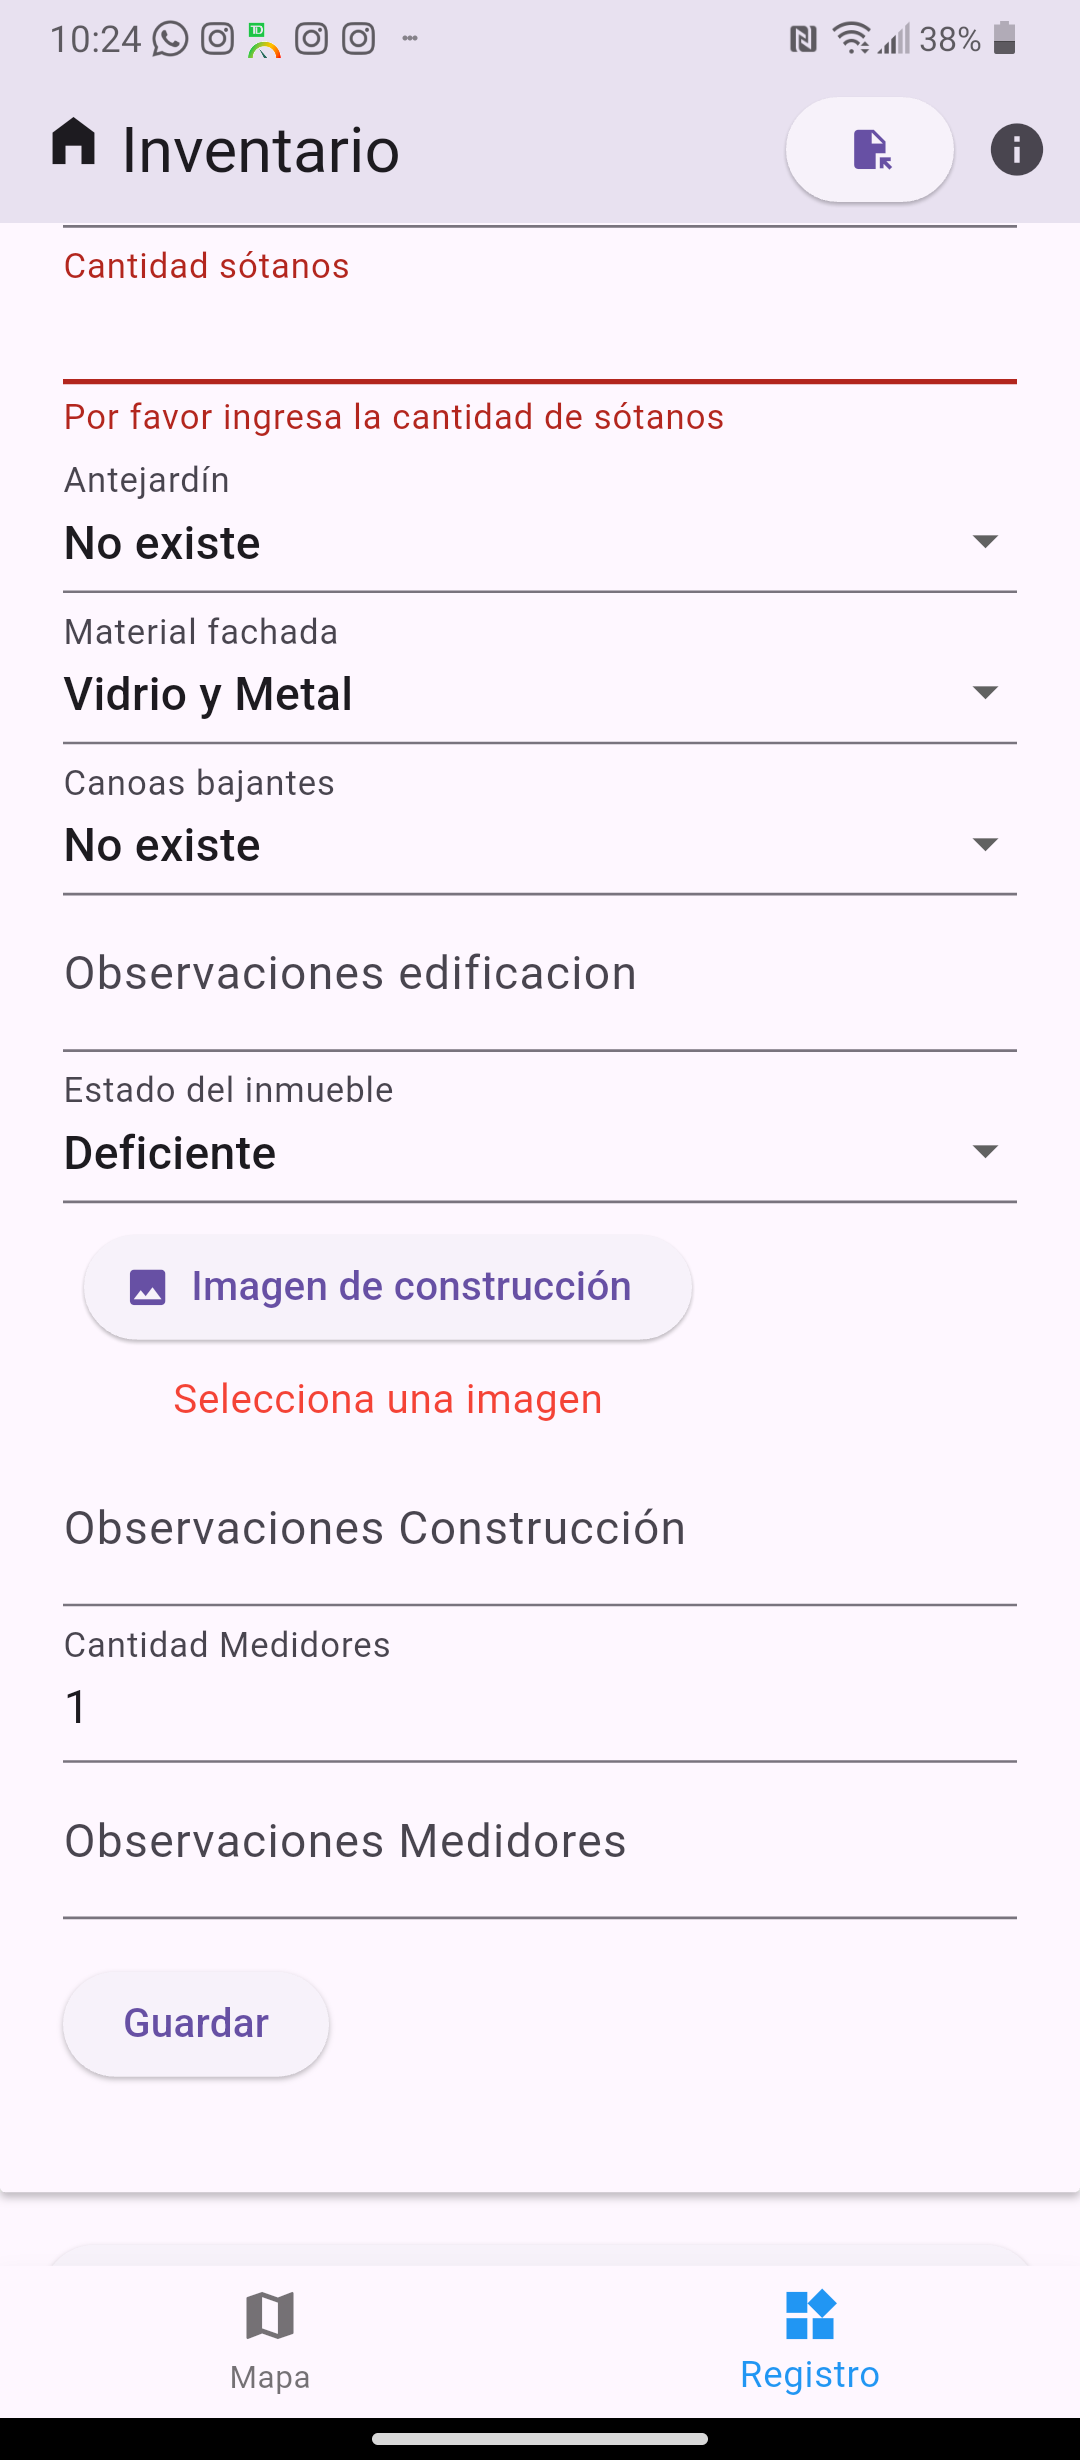
\includegraphics[width=0.3\textwidth]{Graphics/Capitulo 4/LG Android 13/4.4/2.png}
    \caption{Prueba de validación de formularios}
    \label{fig:figura22}
\end{figure}

En esta prueba se pueden ver varios escenarios del proceso de validación de los subformularios. Los campos que se marcaron en rojo no se rellenaron a propósito con el objetivo de mostrar que la
validación funciona. La aplicación sigue teniendo el comportamiento esperado en las tres versiones de Android

\pagebreak
\section{Edición, recuperación y eliminación de Propiedades y Edificios}
\begin{figure}[h]
    % \centering
    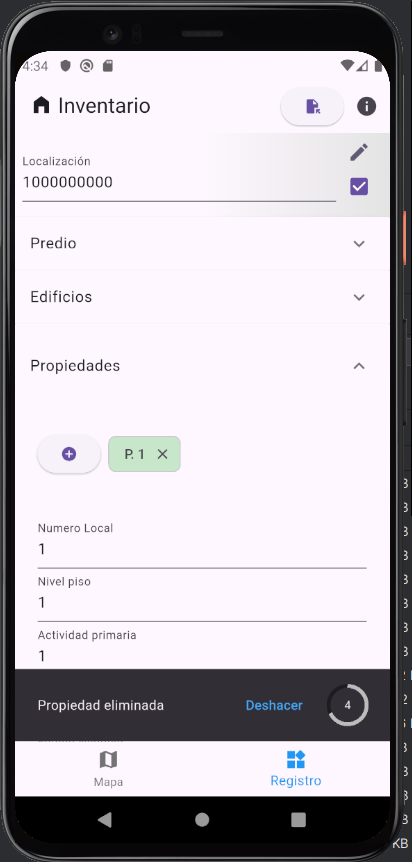
\includegraphics[width=0.3\textwidth]{Graphics/Capitulo 4/Pixel 4 [emulador]/4.5/5.png}
    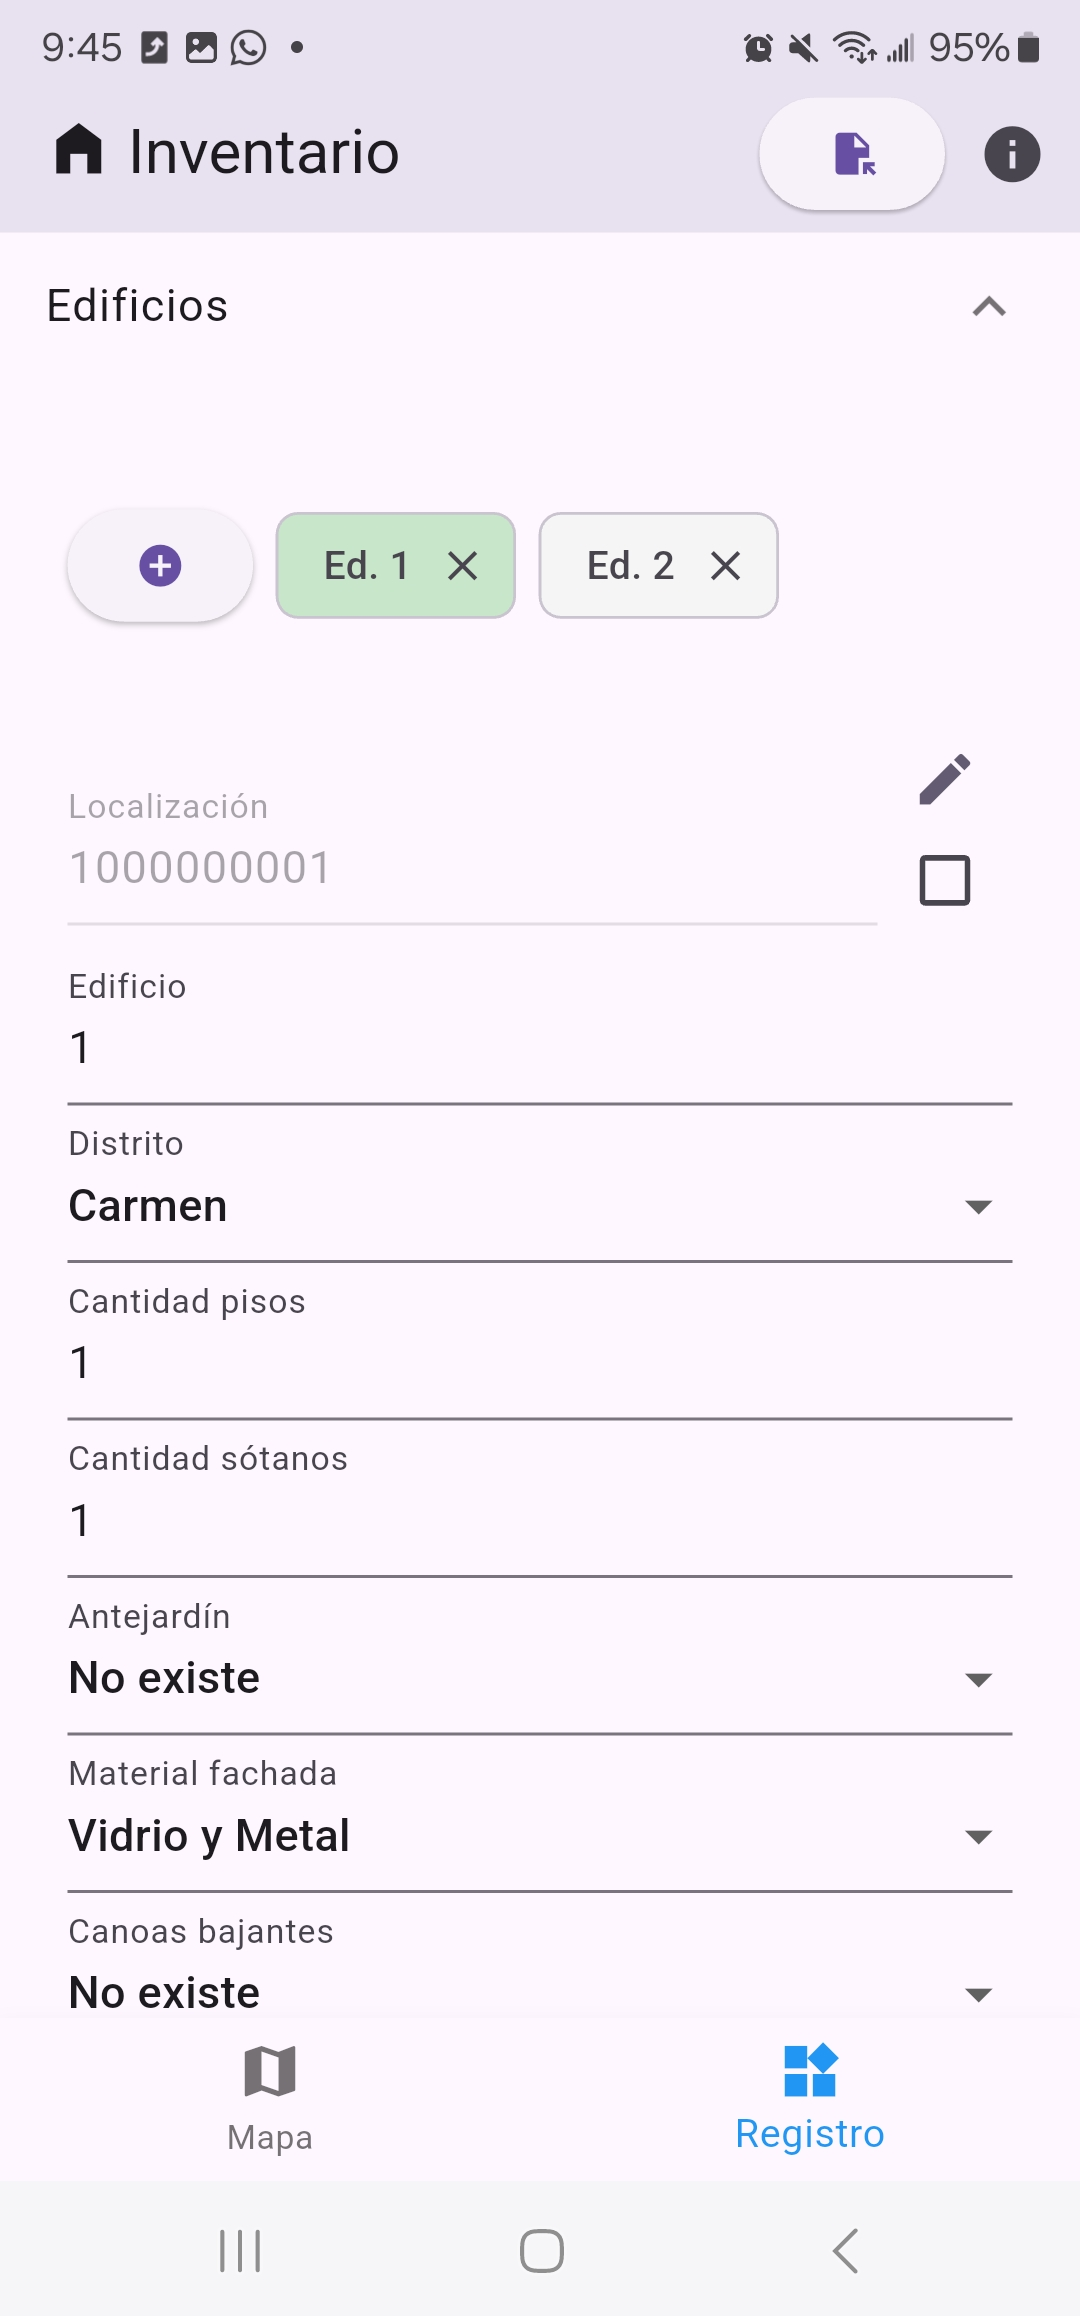
\includegraphics[width=0.3\textwidth]{Graphics/Capitulo 4/Galaxy S23 Ultra Android/4.5/1.jpg}
    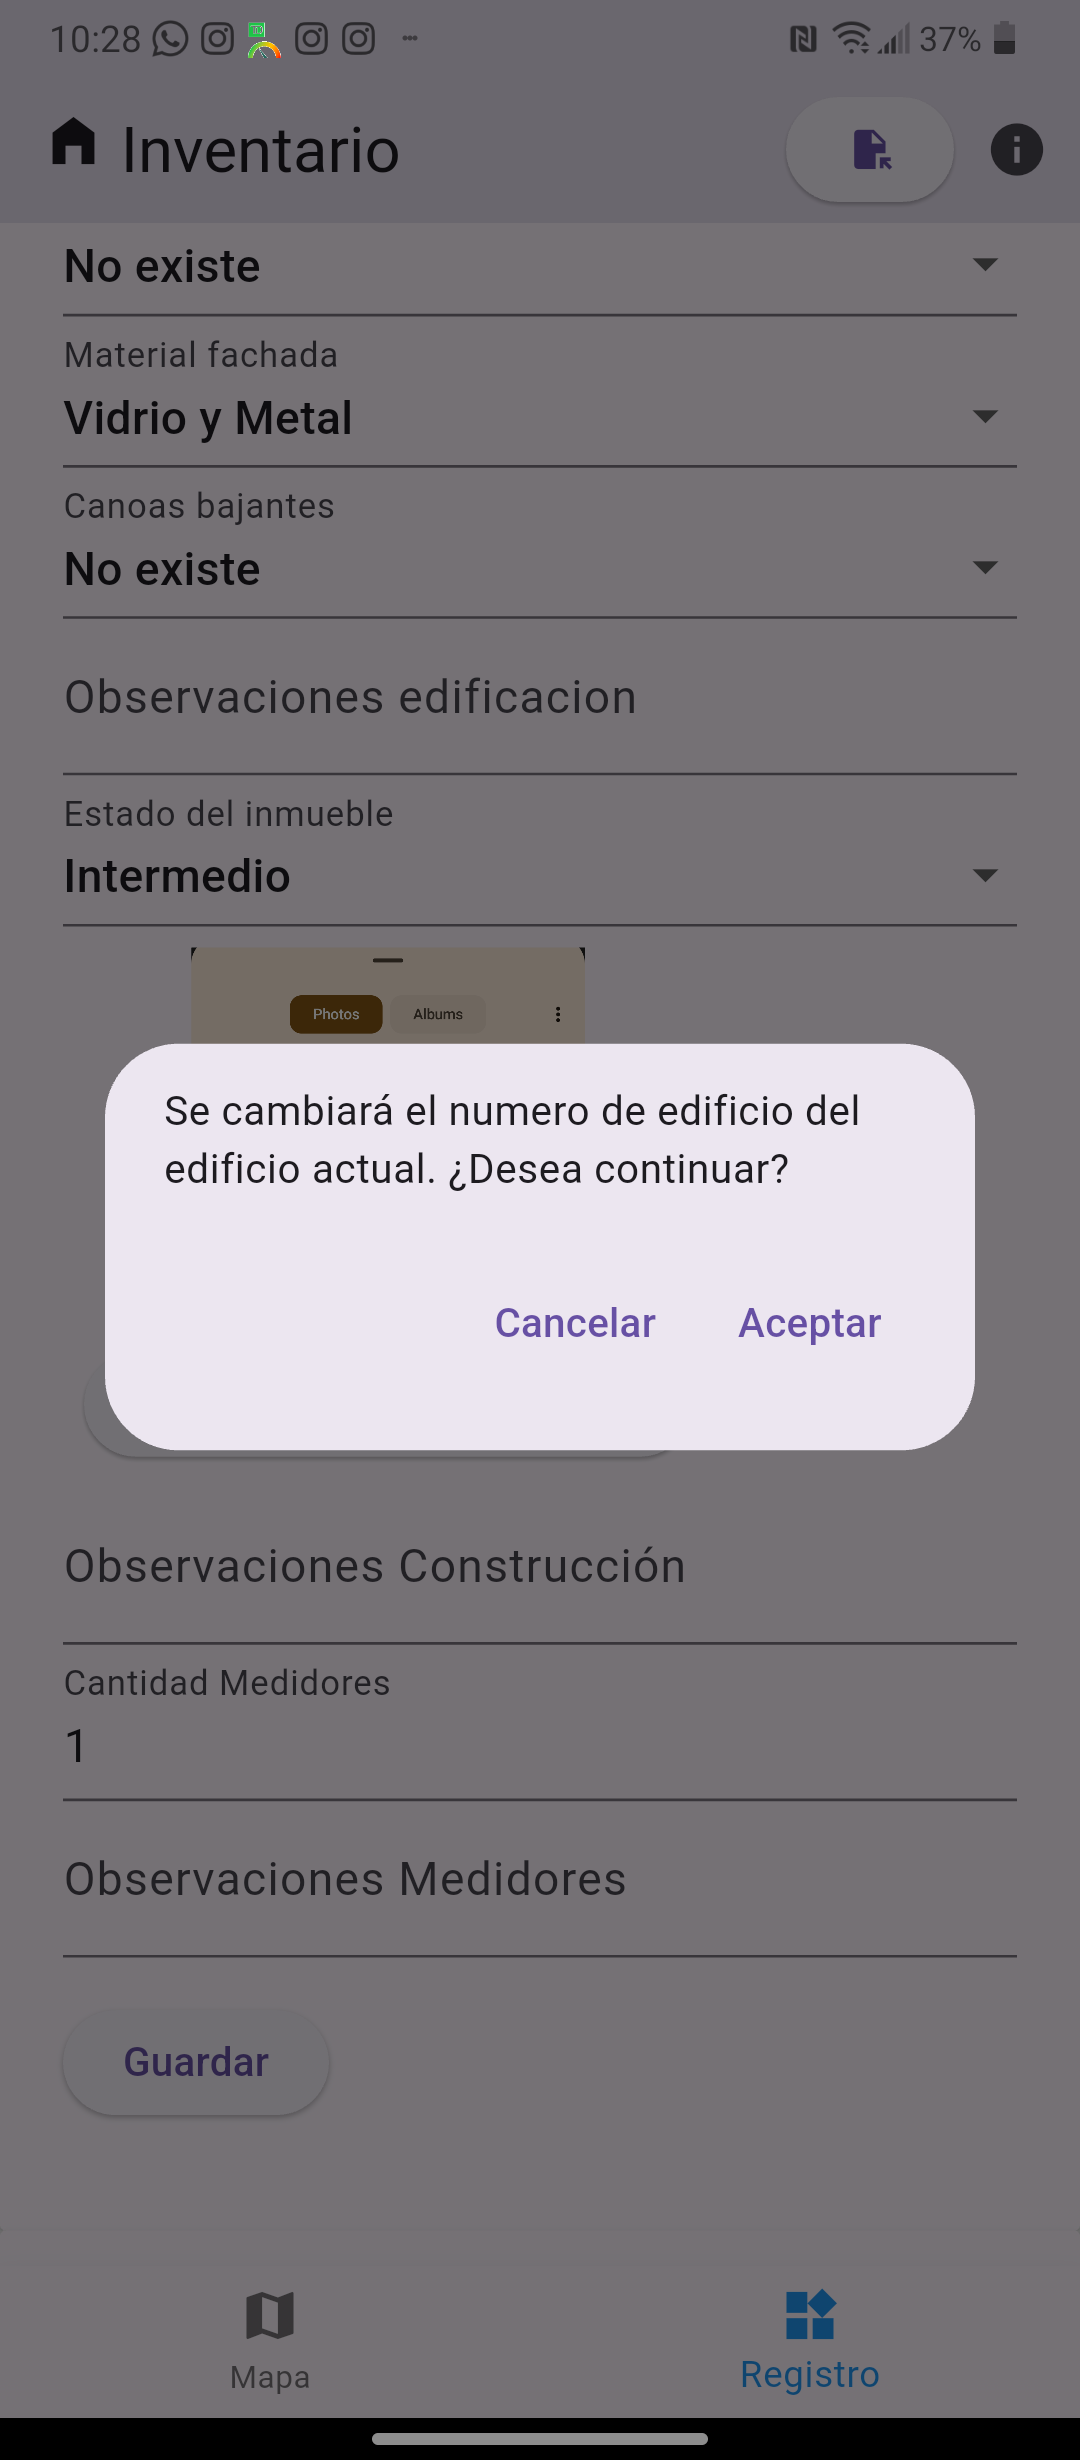
\includegraphics[width=0.3\textwidth]{Graphics/Capitulo 4/LG Android 13/4.4/4.png}
    \caption{Prueba de edición, recuperación y eliminación de Edificios y propiedades}
    \label{fig:figura23}
\end{figure}

En la figura \ref{fig:figura23} se aprecian varios escenarios de edición, eliminación y recuperación de datos de propiedades y edificios. En la imagen de la extrema derecha
se observa un mensaje de confirmación ya que se optó por cambiar el número de edificio de un edificio existente, lo cual es una accion no natural y por ende se agrega un paso de confirmación.
En la imagen de la izquierda, podemos apreciar la eliminación de una entidad. Ya sea Edificio o Propiedad, al eliminar alguna entidad, se eliminará al final de un contador que da la oportunidad
de deshacer la eliminación.

\pagebreak

\section{Marcando varios predios como visitados}
\begin{figure}[h]
    \centering
    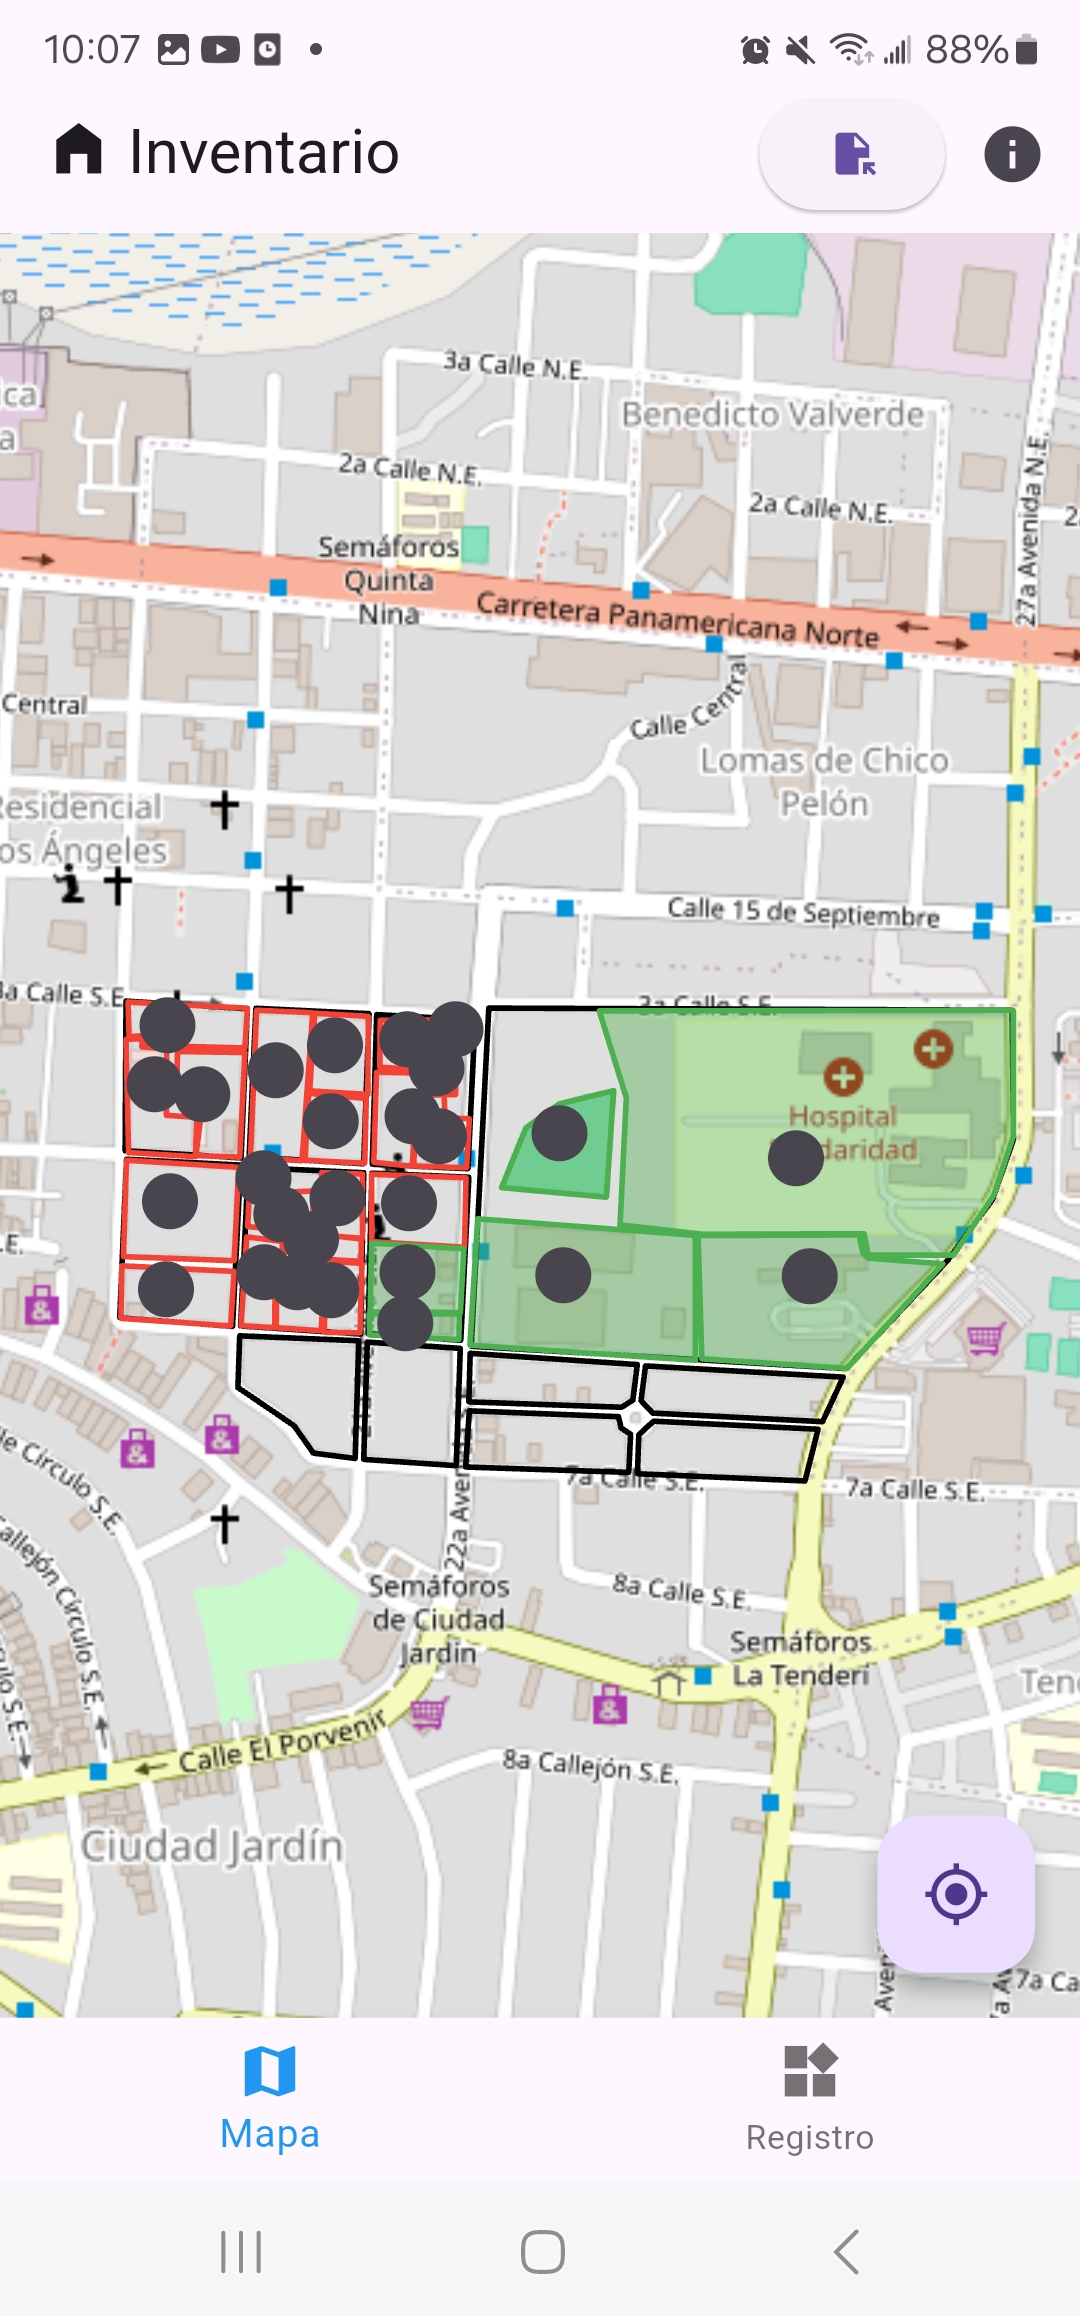
\includegraphics[width=0.3\textwidth]{Graphics/Capitulo 4/Galaxy S23 Ultra Android/4.6/1.jpg}
    \caption{Prueba de la funcionalidad de marcar predios como visitados}
    \label{fig:figura24}
\end{figure}
En la figura \ref{fig:figura24} se pueden observar algunos predios con fondo y bordes verdes, estos fueron marcados como visitados!
\pagebreak
\section{Exportación y Limpieza de la Base de Datos}
\begin{figure}[h]
    \centering
    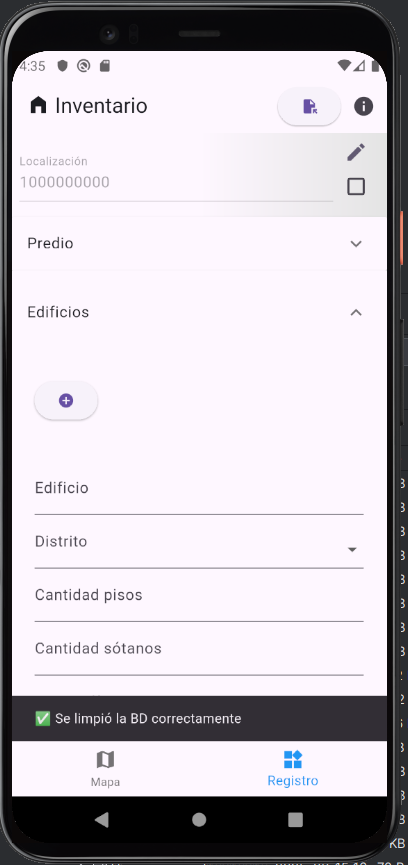
\includegraphics[width=0.3\textwidth]{Graphics/Capitulo 4/Pixel 4 [emulador]/4.7/1.png}
    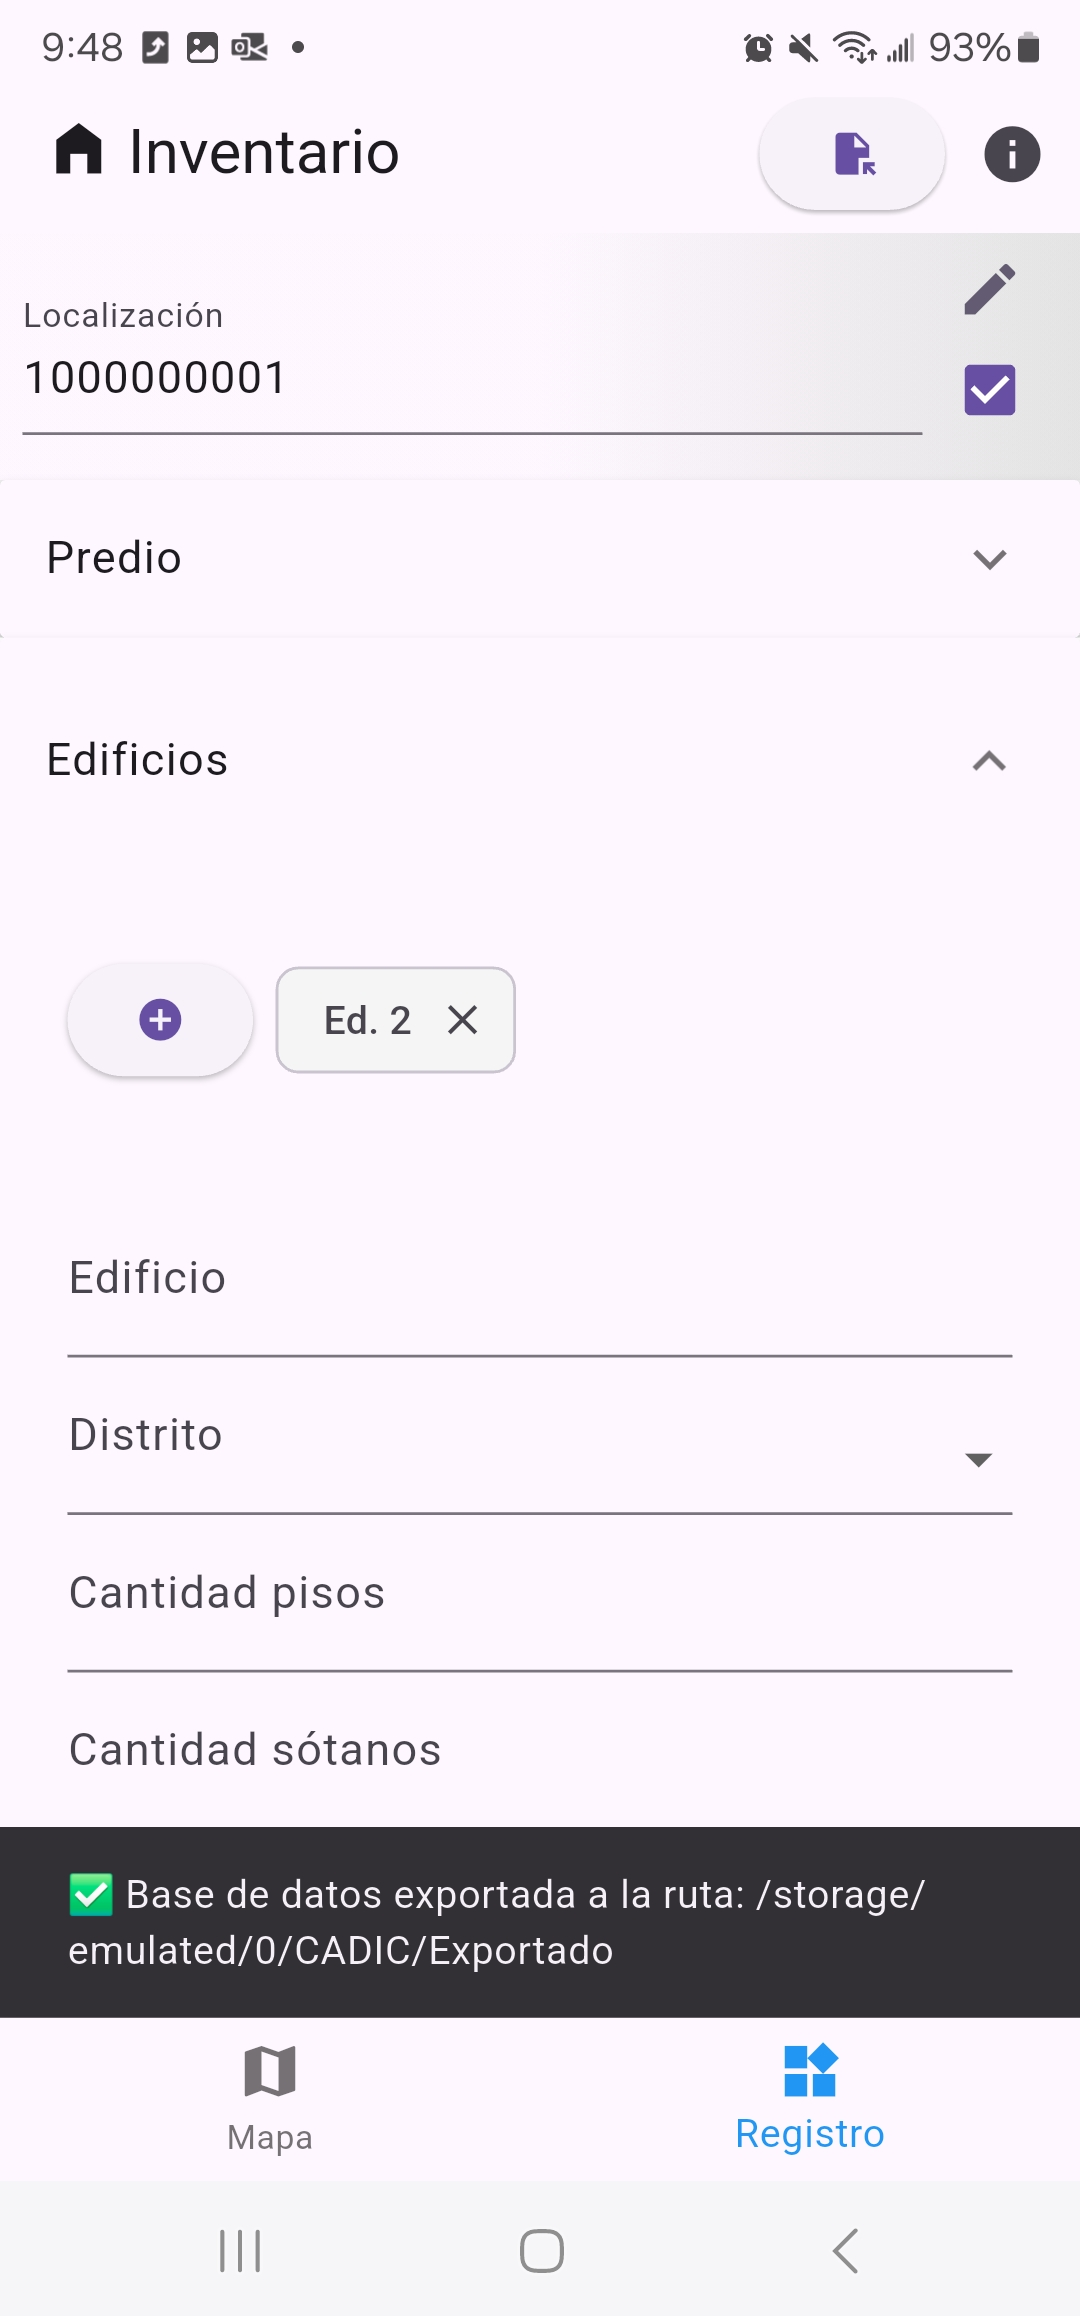
\includegraphics[width=0.3\textwidth]{Graphics/Capitulo 4/Galaxy S23 Ultra Android/4.7/1.jpg}
    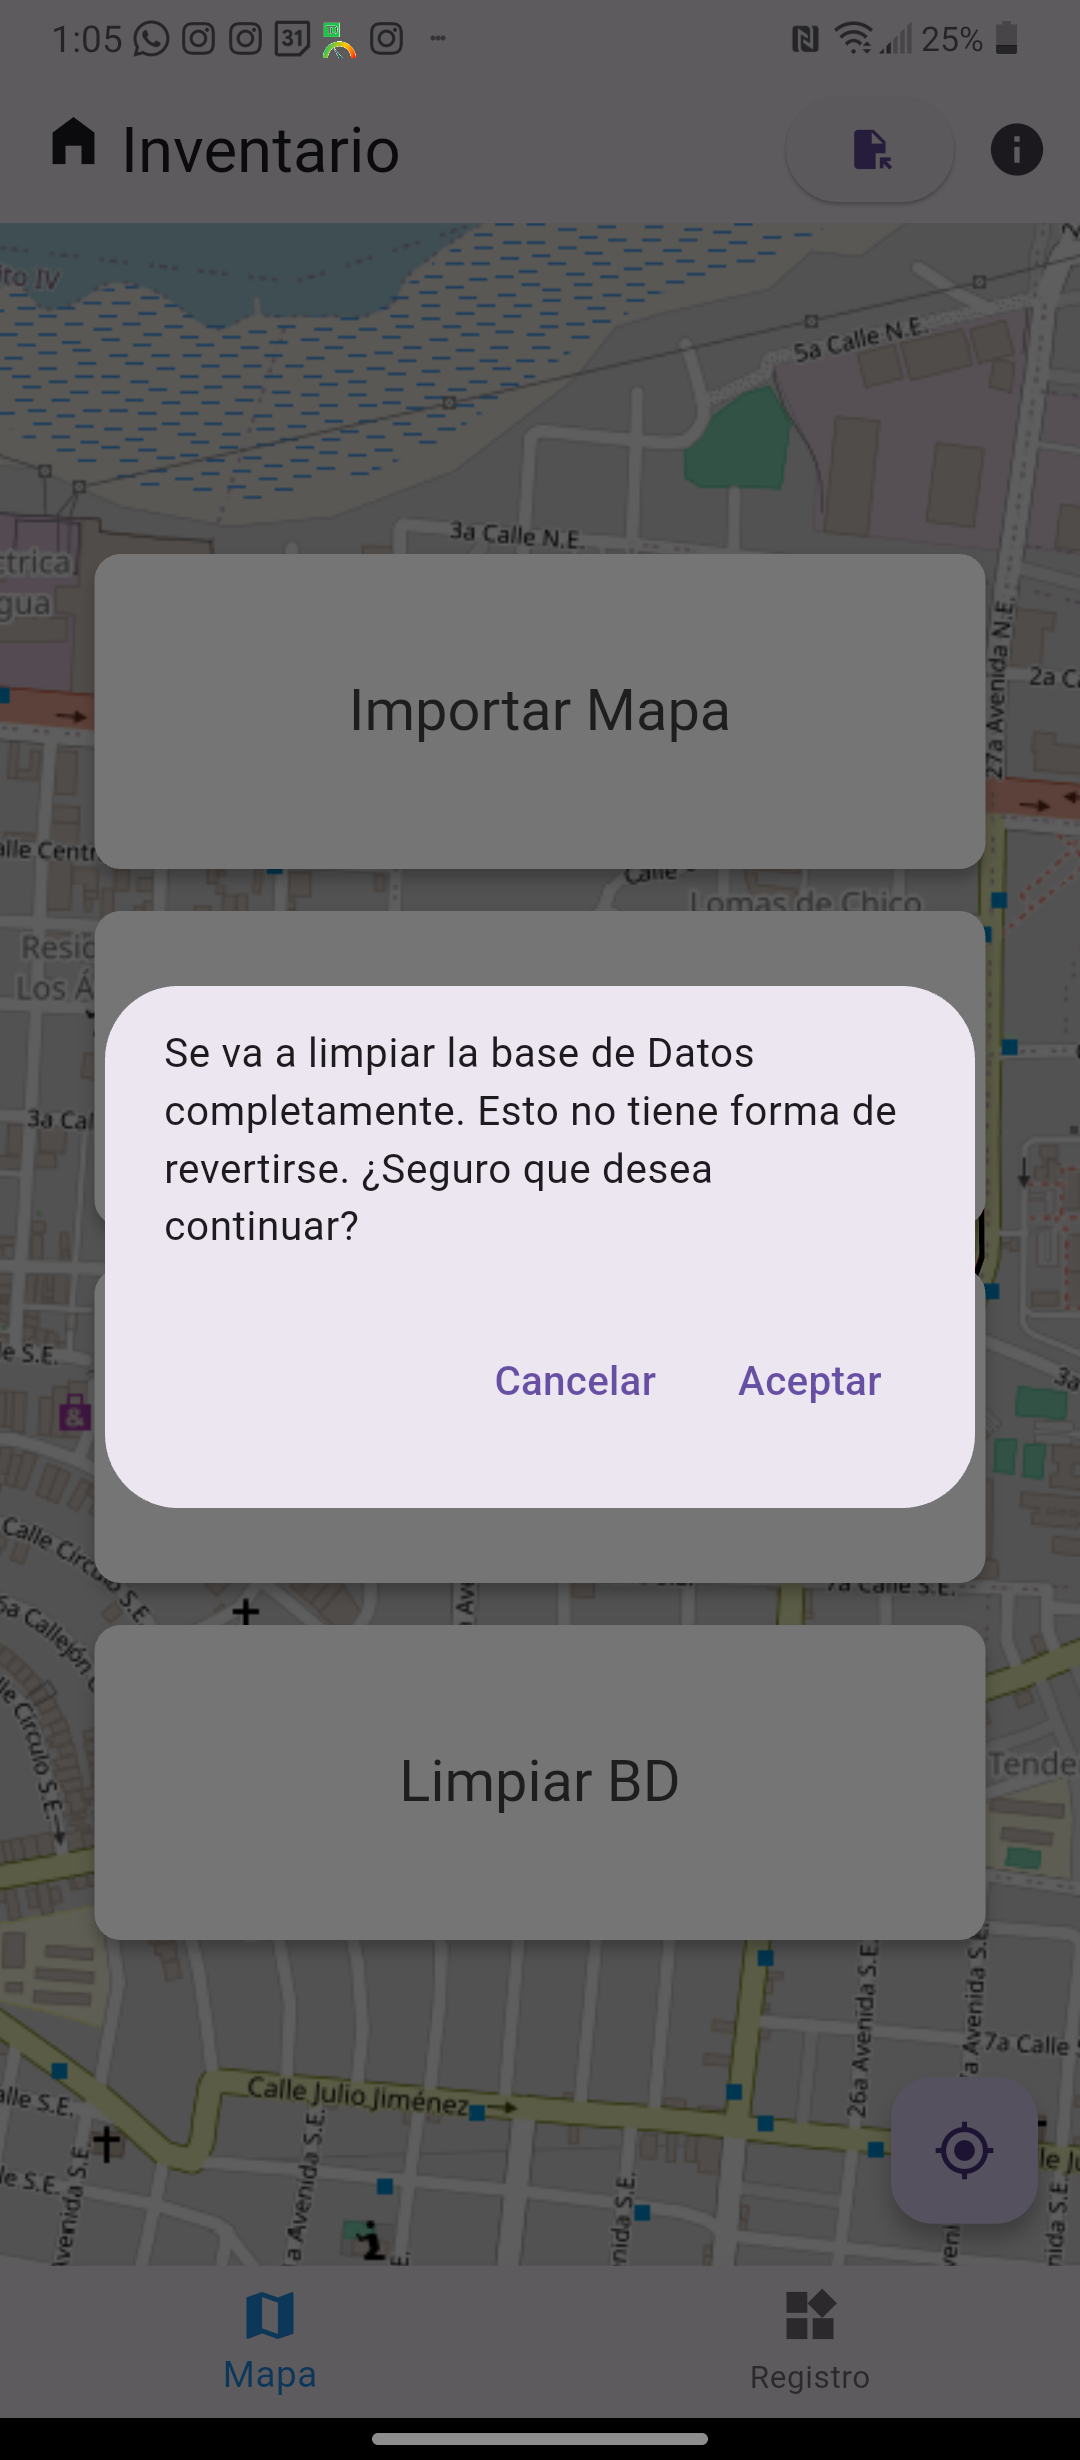
\includegraphics[width=0.3\textwidth]{Graphics/Capitulo 4/LG Android 13/4.7/Screenshot_20250615-130550.png}
    \caption{Prueba de la funcionalidad de marcar predios como visitados}
    \label{fig:figura25}\
    Recalcar que siempre se exporta la base de datos a la misma ruta/directorio: 'CADIC/Exportado' y también importante recalcar que al limpiar la base de datos se eliminan todas las tablas
    excepto la que guarda el nombre del encuestador que está usando la aplicación.
\end{figure}

